\chapter{Detector Physics}\label{chapter:DetectorPhysics}
\section{Particle Detectors}
Particle detectors for high-energy physics experiments typically include a number of components, each designed to perform one specific task. A common design, based on a central interaction region (i.e. in collider experiments) uses a fine-grained tracker close to the interaction region, with calorimeters and coarse trackers further out. Muon chambers around the outside provide a signal if a particle penetrates the calorimeters and leaves the detector entirely. In this scenario, detector elements are designed to perform either tracking or calorimetry. A tracker provides details of the passage of ionising particles through a detector, usually in the form of spatial points or \emph{hits}. Hits are combined using a track reconstruction algorithm, yielding parameters which estimate the path a particle took (usually a straight line, or a curve or helix in a magnetic field). Tracks may be back-projected to estimate the interaction vertex, and curvature in a magnetic field provides a measurement of particle momentum\citep{Green2008}. 

The history of tracking detectors began with the bubble chamber, in which each event consists of images of the bubbles produced when ionising particles pass through a detector, recorded onto photographic plates. The signal readout was performed by manually scanning each photographic plate. Wire chambers and drift chambers also provide this tracking capability, and they are preferred since the readout is electronic, and can be automated. In a drift chamber, ionising particles release electrons from the gas that fills the chamber. These electrons drift in an electric field (provided by field wires) towards a signal wire where the charge is read out. The position resolution of such a detector depends on the wire pitch. The current generation of particle physics experiments also makes use of Silicon trackers, which use the properties of Silicon semiconductors to trap ionisation charge into pixels which can be read out electronically. These can provide extremely high resolution (on the order of $\micron$) but are also rather expensive.

Calorimeters deal with the determination of the kinetic energy of a particle (or of an electromagnetic or hadronic shower produced by an initial particle). The energy losses are measured by a detector medium which produces light or charge signals proportional to the energy deposited. With a sufficiently large calorimeter, particles of interest will come to a stop completely within the calorimeter, and the total kinetic energy can be measured. Liquid Argon is currently used in the calorimeters of a number of experiments, including the electromagnetic calorimeter of the ATLAS\citep{ATLAS1999} experiment. Liquid Argon is usually used to build sampling calorimeters, in which layers containing liquid Argon are alternated with layers of a high-density absorber such as Lead. This technology provides calorimetry in conjunction with high stopping power. The scintillation light from the liquid Argon is generally wavelength shifted in order that the peak wavelength coincides with the peak photon detection efficiency of a photosensitive device. Liquid Argon calorimetry is therefore a demonstrated and proven technology\citep{Aprile2006}.

\section{Physics Motivation}
Many of the fundamental results of experimental neutrino physics have been provided by large underground neutrino detectors such as SNO and Super-Kamiokande. These couple a large target mass with the shielding that several hundred metres of rock provides against many sources of background events (cosmic rays, for instance). The next generation of experiments will require an order of magnitude increase in detector size to reach new physics goals.

A large, high-mass detector on the order of $100\kton$ to $1\Mton$ would provide sensitivity for a number of new scientific opportunities, including a precision measurement of the neutrino mixing angle $\theta_{13}$ as well as sensitivity to the $\Charge\Parity$ violating phase $\delta$ (and hence to leptonic $\Charge\Parity$ violation measurements). In addition to this conventional neutrino physics programme, such a detector would be able to study neutrinos from supernovae, permitting studies of the mechanisms of the explosions, as well as having a sensitivity to proton decay with lifetimes of up to $10^{35}$ years, a number of significance to several theoretical models\citep{Laguna2009}.

\section{Liquid Argon Time Projection Chambers}
Ionising radiation moving through \ac{LAr} generates both ionisation charge and scintillation light signals, though the energy resolution of the scintillation light is typically poor compared to that of the ionisation charge, since only a small number of the emitted photons can usually be detected\citep{Aprile2006}. \aclp{LAr TPC} were first proposed by Carlo Rubbia in 1977\citep{Rubbia1977}, when he noted that \ac{LAr} has several useful properties as a detector medium, including high density, long electron drift times, and relatively high abundance making it cheap to obtain in large quantities.

The ionisation charge produced by a primary ionising particle can be drifted through an applied electric field to a readout plane (anode), see fig. \ref{fig:tpc-schematic}.

\begin{figure}
\centering
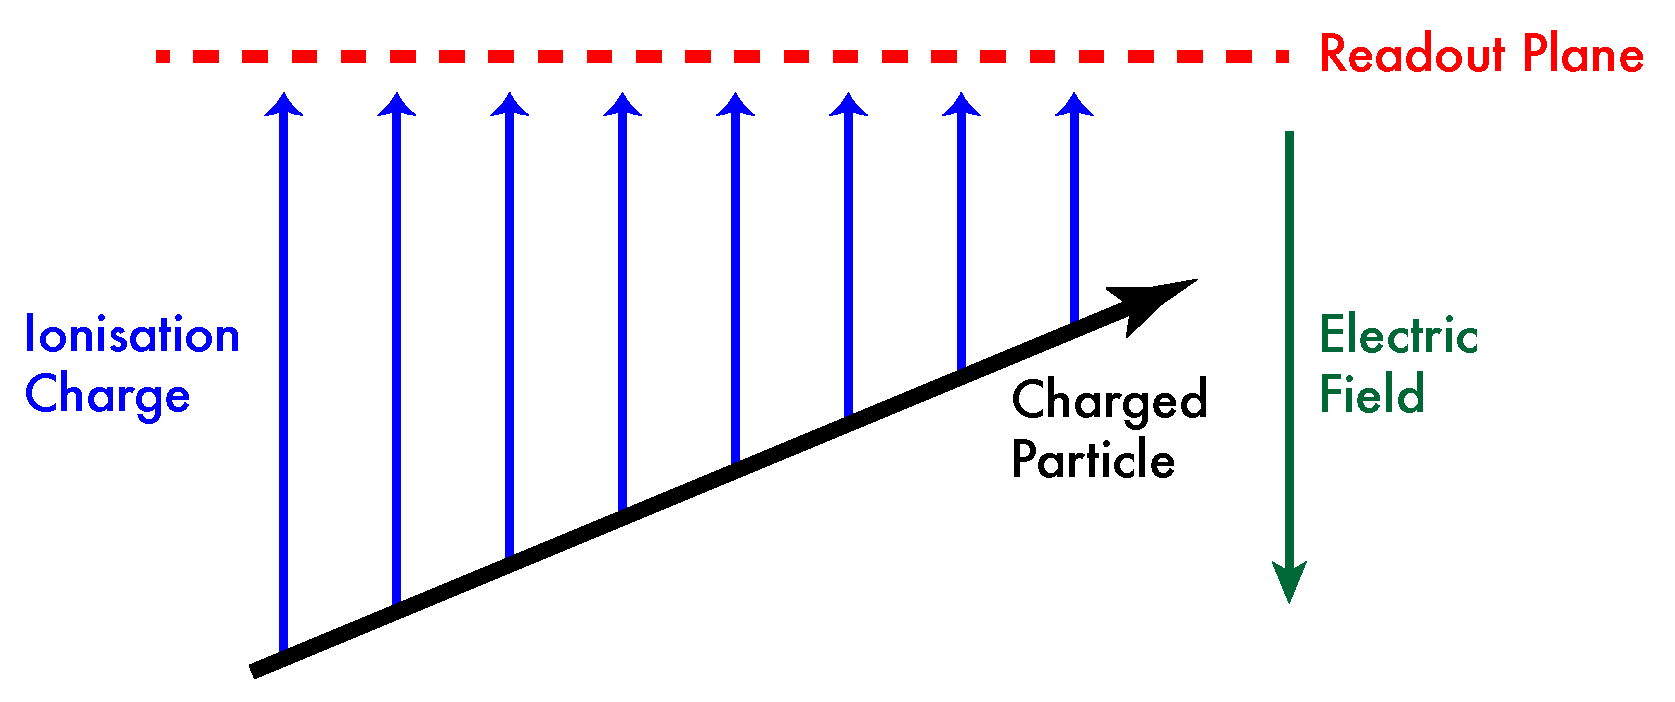
\includegraphics[width=\textwidth]{chapters/detectorphysics_images/TPC-Schematic}
\caption[Schematic diagram of the operation of a time-projection chamber]{\label{fig:tpc-schematic}Schematic diagram of the operation of a time-projection chamber. An incident ionising particle produces ionisation charge, which drifts in an applied electric field to a readout plane. The readout plane provides a two-dimensional $(x,y)$ position measurement, and the depth $z$ can be determined from the drift time $t$ taken for charge to arrive at the readout plane.}
\end{figure}

\subsection{Production of Ionisation Charge}\label{sec:production-ionisation-charge}
The amount of ionisation charge $Q$ that drifts to a readout plane is smaller than that initially produced by the passage of an ionising particle $Q_0$, since some of the electron-ion pairs undergo recombination processes, i.e. $Q = \mathcal{R}Q_0$ with some \emph{quenching factor} $\mathcal{R}$. The recombination is described empirically by Birk's Law\citep{Birks1964}:
\begin{equation}\label{eqn:birks_law}
    Q = \frac{Q_0}{1 + k_E / \epsilon}
\end{equation}
where $k_E$ is a recombination constant, to be fitted to data, and $\epsilon$ is the applied electric field strength. In terms of the stopping power $dE/dx$, this is written:
\begin{equation}\label{eqn:birks_law_dEdx}
    Q = \frac{Q_0}{1 + k_Q\, dE/dx}
\end{equation}
with $k_Q(\epsilon) = k_E / \epsilon$.

The {\sc Icarus} experiment\citep{Amoruso2004} measured the quenching factor $\mathcal{R}$ as a function of the applied field and $dE/dx$, finding $\mathcal{R} = 0.71$ for $dE/dx$ from minimum ionising particles up to $\sim 30 \MeV \gram^{-1} \cm^2$ in an applied field of $0.5 \kvolt \cm^{-1}$. They found, however, that their data was best described with an additional normalisation constant $A$:
\begin{equation}\label{eqn:icarus_quenching}
Q = A\frac{Q_0}{1 + k_E/\epsilon \, dE/dx}
\end{equation}
with $A=0.800\pm0.003$ and $k_E = 0.0486\pm 0.0006 \kvolt \cm^{-1}$. This updated quenching factor has been applied in the Warwick \emph{Lamu} simulation package for liquid Argon detectors (see section \ref{sec:lamu} for further details).

\subsection{Drifting Charge}
Charge transport through a medium such as \ac{LAr} is governed by the mobility $\mu$ of charge carriers (electrons)\citep{Aprile2006}. The drift velocity $\vec{v}$ is:
\begin{equation}\label{eqn:charge_transport}
    \vec{v} = \mu \vec{E}
\end{equation}
where $\mu$ is constant for low electric fields $\vec{E}$. An electron is considered to be \emph{quasifree} when the mobility in the absence of an electric field $\mu_0 > 10 \cm^2 \volt^{-1} \second^{-1}$. For \ac{LAr}, where $\mu_0 = 625 \pm 15 \cm^2 \volt^{-1} \second^{-1}$\citep{Aprile2006}, the drift velocity is large and drift lengths are limited primarily by impurities in the Argon, which capture the charge.

Another constraint on the drift length is the reduction in spatial resolution due to \emph{transverse diffusion} of drifting charge. As the charge drifts from the point of creation to the readout plane, diffusion perpendicular to the direction of motion acts to spread out the electron cloud. For long drift lengths, this reduces the $xy$ resolution which can be achieved at the readout plane.

\subsection{Wire Readout}
In most current and planned \acsp{TPC} the readout plane consists of a grid of wires, attached to charge amplifiers and subsequent electronics to read the charge signal that collects on each wire. Coincidence of signals on $x$ and $y$ wires provides a two-dimensional view of charge arriving at the readout plane. The {\sc Icarus} T600\citep{Amerio2004} detector, with a $500\ton$ fiducial mass, demonstrated the success of wire plane readout on a small scale. Projects including MODULAr\citep{Baibussinov2008} plan to carry the concept to larger detectors by grouping many {\sc Icarus}-style modules together. Alternative plans by collaborations such as LANNDD\citep{Cline2003} use a single \ac{LAr} volume, internally segmented by readout planes.

Whilst the wires are inexpensive, large wire plane detectors require many electronics (readout) channels, each of which carries significant cost. For a $100\kton$ detector, this cost is substantial, and can be reduced only by using longer wires (which requires higher tension in the wires themselves, and presents an engineering challenge) or by increasing the inter-wire spacing, thus reducing the spatial resolution of the detector. Another option would be to increase the drift length, but this also results in degraded spatial resolution due to transverse diffusion of charge as it drifts.

\subsection{Thick Gas Electron Multipliers}
A \ac{TGEM} is a \ac{PCB} of thickness on the order of $1\mm$, with copper cladding on both sides. Holes are drilled into the \ac{PCB} at regular intervals, with diameters on the order of $1\mm$ and spaced by $< 1\mm$. The holes may be further shaped by etching e.g. to smooth rough edges from the drilling process. An electric potential is applied across the two Copper electrodes, creating a strong field in the holes and extending into the region around them. Electrons arriving at the \ac{TGEM} are focused into the holes by this field. The high field strength ($> 1.5 \kvolt \mm^{-1}$) within the holes causes rapid acceleration of the electrons.

If the \ac{TGEM} is in gaseous Argon, the accelerated electrons cause ionisation of Argon in the hole, freeing more electrons in an avalanche process. In this way, the \ac{TGEM} acts as a charge multiplier. In liquid Argon, the mean free path of electrons is much shorter than in gas, and the electrons do not gain sufficient energy to ionise an Argon atom (the ionisation energy of Argon is $23.4\eV$\citep{Aprile2006}). Some of the electrons do, however, gain enough energy to excite electrons in Argon atoms ($11.55\eV$ threshold\citep{Stewart2010}), which subsequently emit photons and allow for optical readout of the \ac{TGEM}\citep{Lightfoot2009}.

The light produced by excitation processes in the holes of a \ac{TGEM} immersed in liquid Argon could be imaged and a reconstruction procedure applied to obtain the $(x,y)$ position of the hole(s) in which light was produced. As an alternative to wire plane readout, this optical readout procedure could have a much lower cost, due primarily to a reduction in the number of readout channels required. One approach would be to image a large area (on the order of $1 \metre^2$) with a single \ac{CCD} camera. This scenario is complicated by the necessity to focus the light onto the \ac{CCD}, and the time resolution which could be achieved is limited by the frame rate of the \ac{CCD}. In order for the time resolution to match that of the $xy$ plane, a \ac{CCD} that operates at frequencies of $\sim 1\MHz$ (and with high efficiency in the cold environment of \ac{LAr}) would be required. Such devices do not yet exist.

The second option is to use a sparse array of Silicon photomultipliers. These devices have high quantum efficiency and provide single photon sensitivity. Using a grid of silicon photomultipliers, it is possible to determine the position of a light source based on the relative intensities recorded at several detectors (see section \ref{sec:point-source-recon}).

\section{Point Light Source Reconstruction}\label{sec:point-source-recon}
In order that the position resolution and associated measurement uncertainty associated with reconstructing point light sources on a plane could be estimated, I wrote a simulation that produces a \emph{flux map} for a detector plane some distance $\Delta z$ from a plane of point light sources. This detector flux map is then used to calculate the integrated light intensity seen by a photosensitive device with a given area, active area and quantum efficiency. Such device areas can be positioned on the detector plane, and the output from the simulation then provides a list of intensities at each detector from a given distribution of sources. A visualisation of this output is show in fig. \ref{fig:flux-example}.

\begin{figure}
\centering
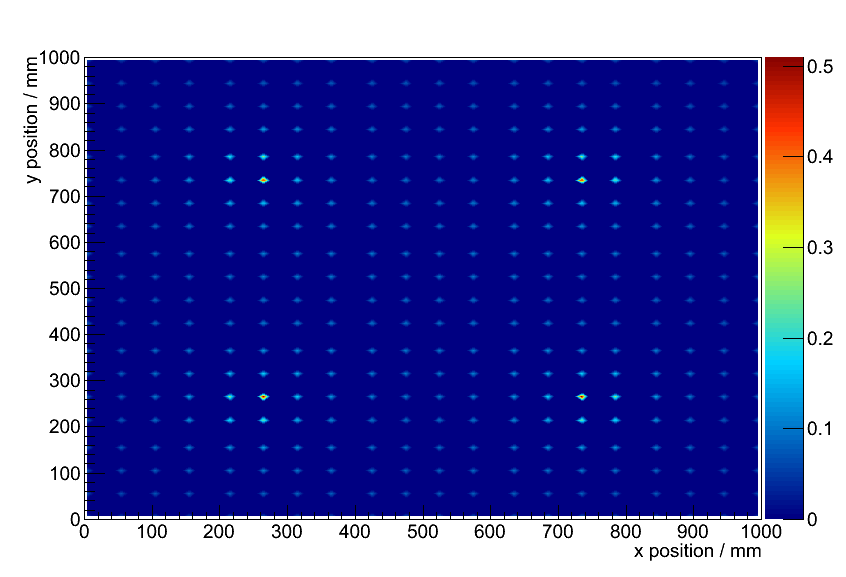
\includegraphics[width=0.85\textwidth]{chapters/detectorphysics_images/four-sources}
\caption[Simulation of light intensity recorded by a sparse array of photodetectors]{\label{fig:flux-example}Simulation of light intensity recorded by a sparse array of photodetectors from four light sources, normalised to the intensity of the sources. The sources are located at $(0.25, 0.25) \metre$, $(0.25, 0.75) \metre$, $(0.75, 0.25)\metre$ and $(0.75, 0.75) \metre$.} 
\end{figure}

This simulation was used by G. Rutter and M. Richards to develop an iterative algorithm for position reconstruction\citep{Rutter2011}. The algorithm requires an initial estimate of the position of a source, which can be obtained from a global approach such as that used to reconstruct position in Anger cameras\citep{Anger1958}. Once this seed position is established, the closest $2\times 2$ square of photosensors surrounding the source is chosen and the reconstructed position iteratively refined by assuming that light from the source propagates freely (i.e. spherically). The ratio of intensities seen by detectors $D_1$ and $D_2$ is given by\citep{Rutter2011}:
\begin{equation}\label{eqn:ratio-detector-intensities}
\alpha = \frac{I_1}{I_2} = \frac{r_2^2}{r_1^2} = \frac{x_2^2 + y_2^2 + h^2}{x_1^2 + y_1^2 + h^2} 
\end{equation}
where the height $h$ is fixed and the coordinates are distances to the detectors $D_1$ and $D_2$. A similar ratio $\beta$ is constructed for detectors $D_1$ and $D_3$. The detector which is shared between the two ratios ($D_1$) is the one which recorded the highest light intensity. The radius $r$ is from source to detector.

Since the inter-detector spacing is fixed, the value of $x_1$ fixes the value of $x_2$, and similarly for the $y$ values. By fixing $x$ values, the $y$ values can be recomputed using equation \eqref{eqn:ratio-detector-intensities}, providing an improved estimate of the $y$ position of the source. This process can be repeated with the $y$ values fixed to improve the $x$ estimate, iteratively converging on the true source position until the difference in coordinates between iterations becomes small compared with other experimental uncertainties (or to a predefined tolerance), see fig. \ref{fig:iterative-source-recon}. The total uncertainty resulting from this procedure is shown as a function of the distance between source and detector planes in fig. \ref{fig:detector-spacing}, where the detectors are arranged in a square grid over a $1\metre^2$ area, with the quoted number of detectors per row, and the reconstruction is of a single point light source. This provides an optimisation procedure for determining the detector coverage required to obtain the desired uncertainty on position resolution.

\begin{figure}
\centering
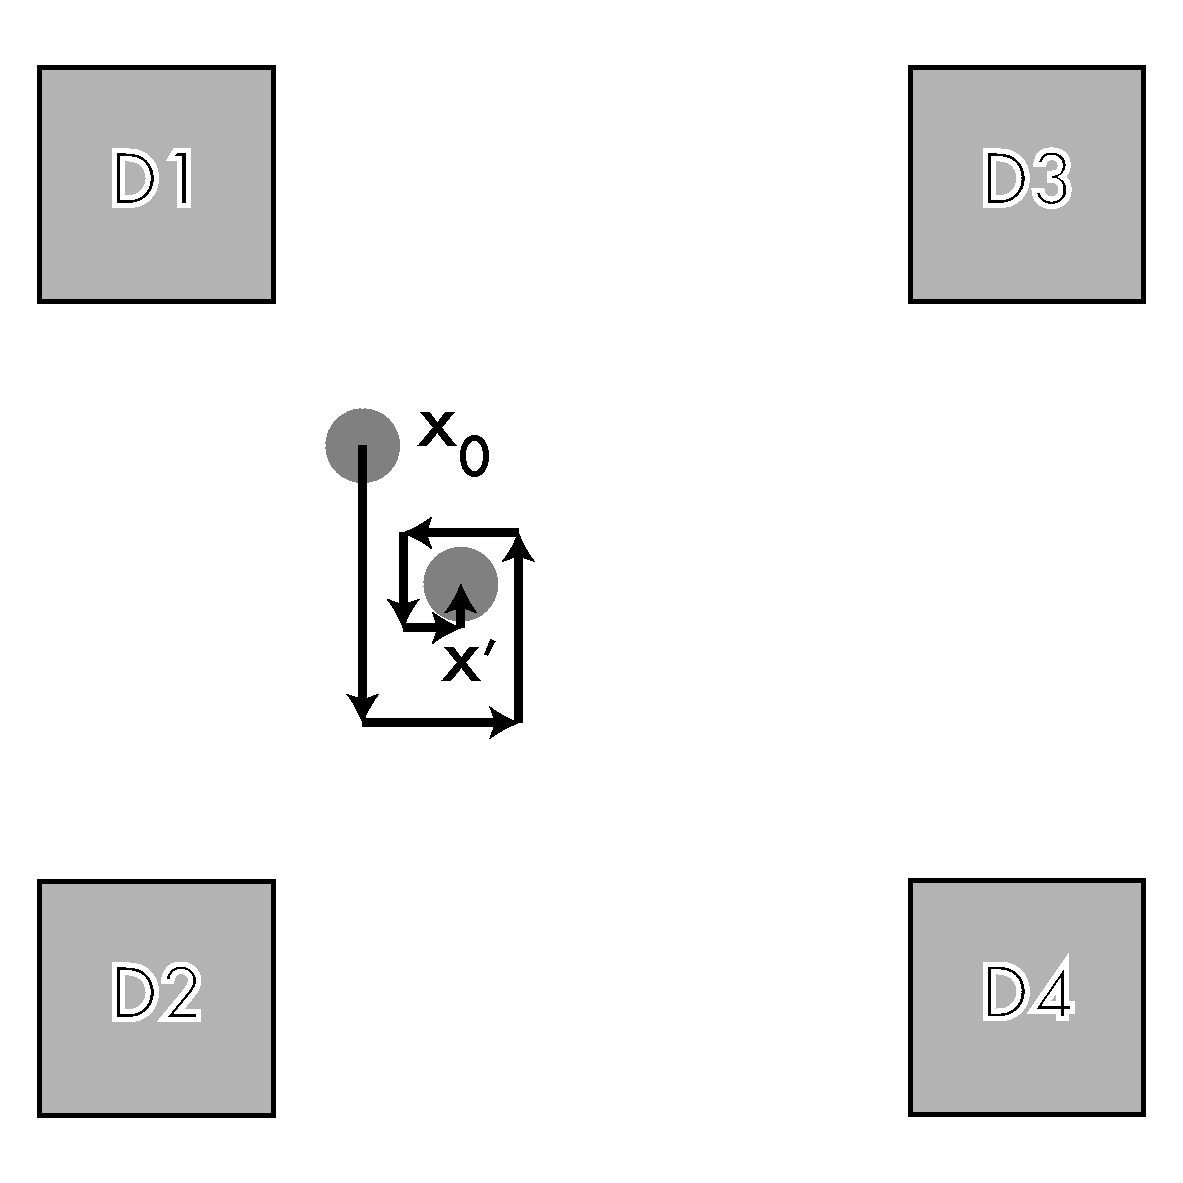
\includegraphics[width=0.5\textwidth]{chapters/detectorphysics_images/Iterative-Source-Recon}
\caption[Iterative point light source position reconstruction]{\label{fig:iterative-source-recon}Iterative reconstruction of the position of a point light source using the ratio of light intensities captured by the surrounding photodetectors. Each step updates either the $x$ or $y$ coordinate by constraining the $y$ or $x$ coordinate and using the known spacing between detectors.}
\end{figure}

\begin{figure}
\centering
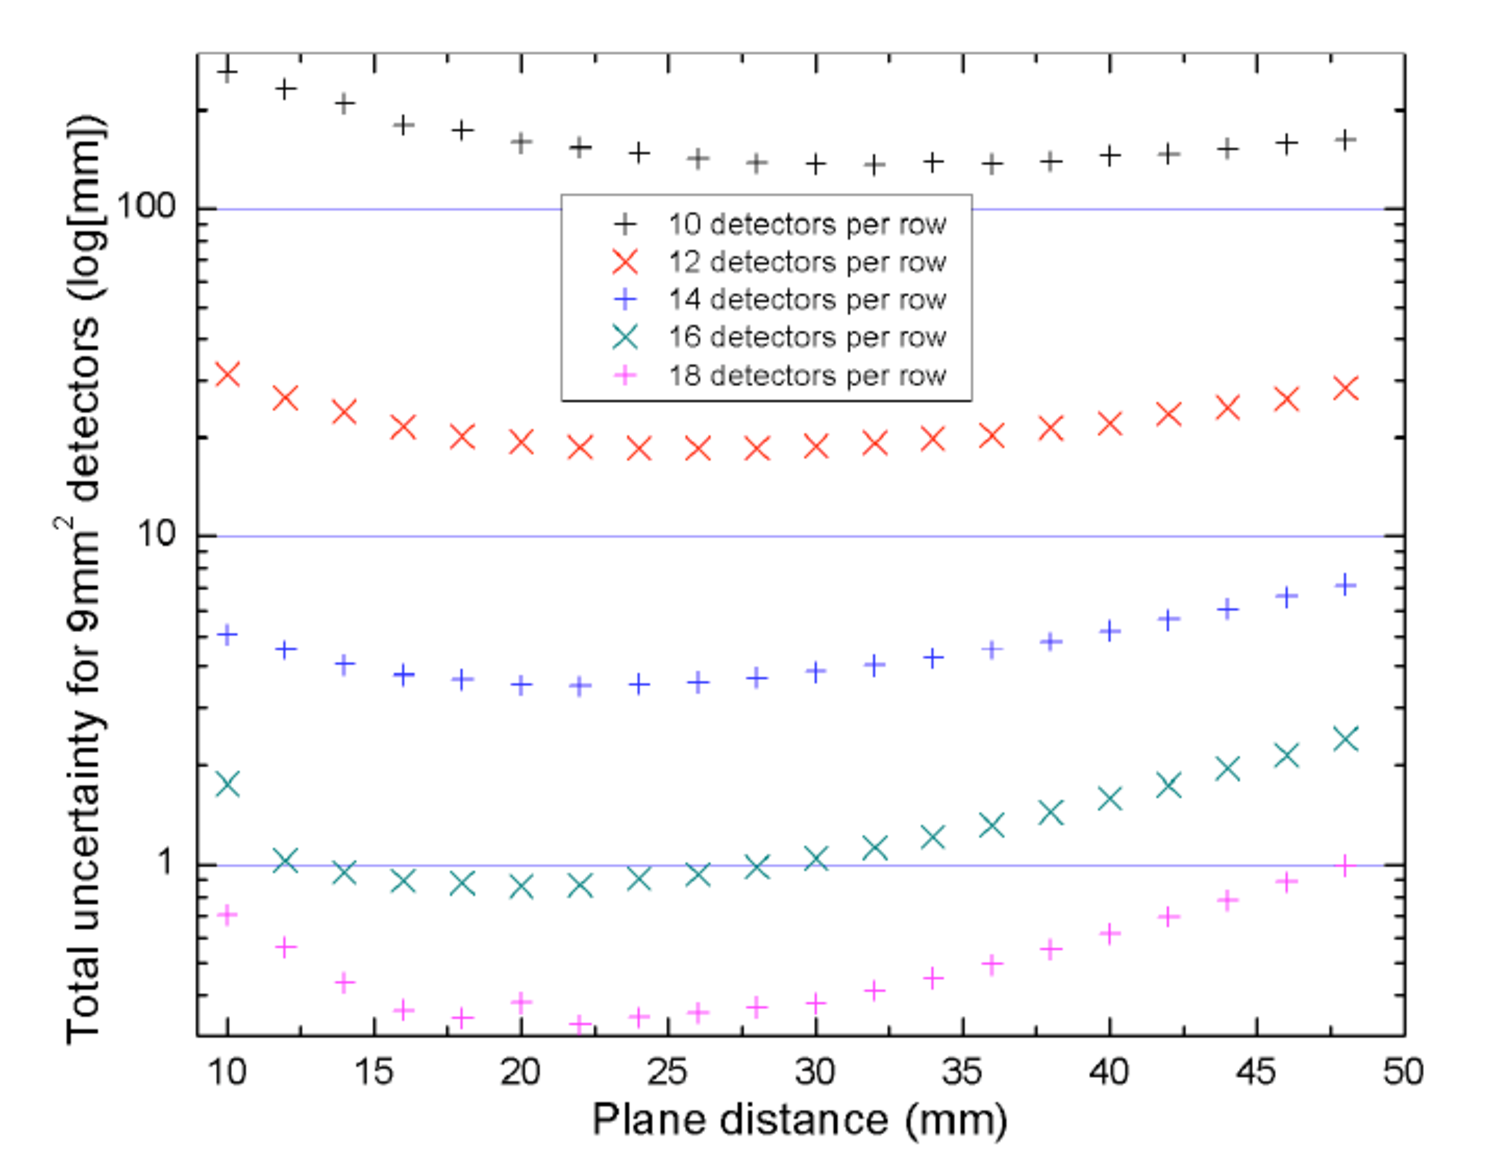
\includegraphics[width=0.6\textwidth]{chapters/detectorphysics_images/detector-spacing}
\caption[Uncertainty on position resolution for several sparse array detector densities]{\label{fig:detector-spacing}The uncertainty on the reconstructed position of a point light source resulting from the iterative procedure discussed in the text, as a function of source--detector plane spacing, for five different sparse array densities (detector--detector spacings). Figure taken from \citep{Rutter2011}.}
\end{figure}

\section{The Lamu Simulation}\label{sec:lamu}
Lamu is a Geant4\citep{Geant4} simulation for liquid Argon volumes which consist of cylinders of configurable radius and height. It includes full modelling of physics processes according to the {\sc qgsp\_bic\_hp} physics list, with all electromagnetic and hadronic processes enabled. The energy loss of particles is modelled taking into account the quenching described in chapter \ref{sec:production-ionisation-charge}, and the \ac{LAr} volume is divided into $(3\times 3\times 3) \mm^3$ cubic voxels. Charged particles are tracked through these voxels to zero energy or until they leave the detector, and the energy deposited in each voxel leads to a mapping between voxel coordinates and the total energy deposited within that voxel. The output from the simulation is this mapping, without any attempt to model drifting charge, readout technologies or subsequent electronics, all of which are dependent on experiment-specific details. The result is a three-dimensional point cloud corresponding to the energy deposition in the detector volume by a particular event. Events are stored in {\sc Root}\citep{Root} files for subsequent analysis.

\subsection{Characterisation \& Testing of the Lamu Simulation}
In order to characterise the Lamu simulation, a number of tests were performed using simulated single particles produced by the Geant4 General Particle Source (GPS) generator\citep{GeantGPS}.

In the first test, muons of fixed kinetic energy were started at the centre of a cylindrical detector volume, with radius $R$ and height $H=2R$. The radius was initially set to $1\metre$ and 100 events were generated. The radially outermost hit in each event was found, and the number of events with such hits lying within $10\cm$ of the detector wall recorded. The radius was increased in $1\metre$ intervals until greater than 95\% of the events were fully contained, i.e. the outermost hit was more than $10\cm$ from the wall. This study was performed at energies from $100\MeV$ to $5000\MeV$ in $100\MeV$ intervals, and the results are shown in fig. \ref{fig:lamu-containment-radius}.

The purpose of this study was to determine the maximum range of a muon of a given energy in liquid Argon, enabling subsequent work to be done in the context of a simulation with geometry chosen so as to fully contain a muon produced at the centre of the detector. For example, $\nu_\mu$ charged current events with an initial neutrino energy of $4500\MeV$ were simulated in a detector of $25\metre$ radius, in order to ensure that the resulting muons were fully contained.

\begin{figure}
\centering
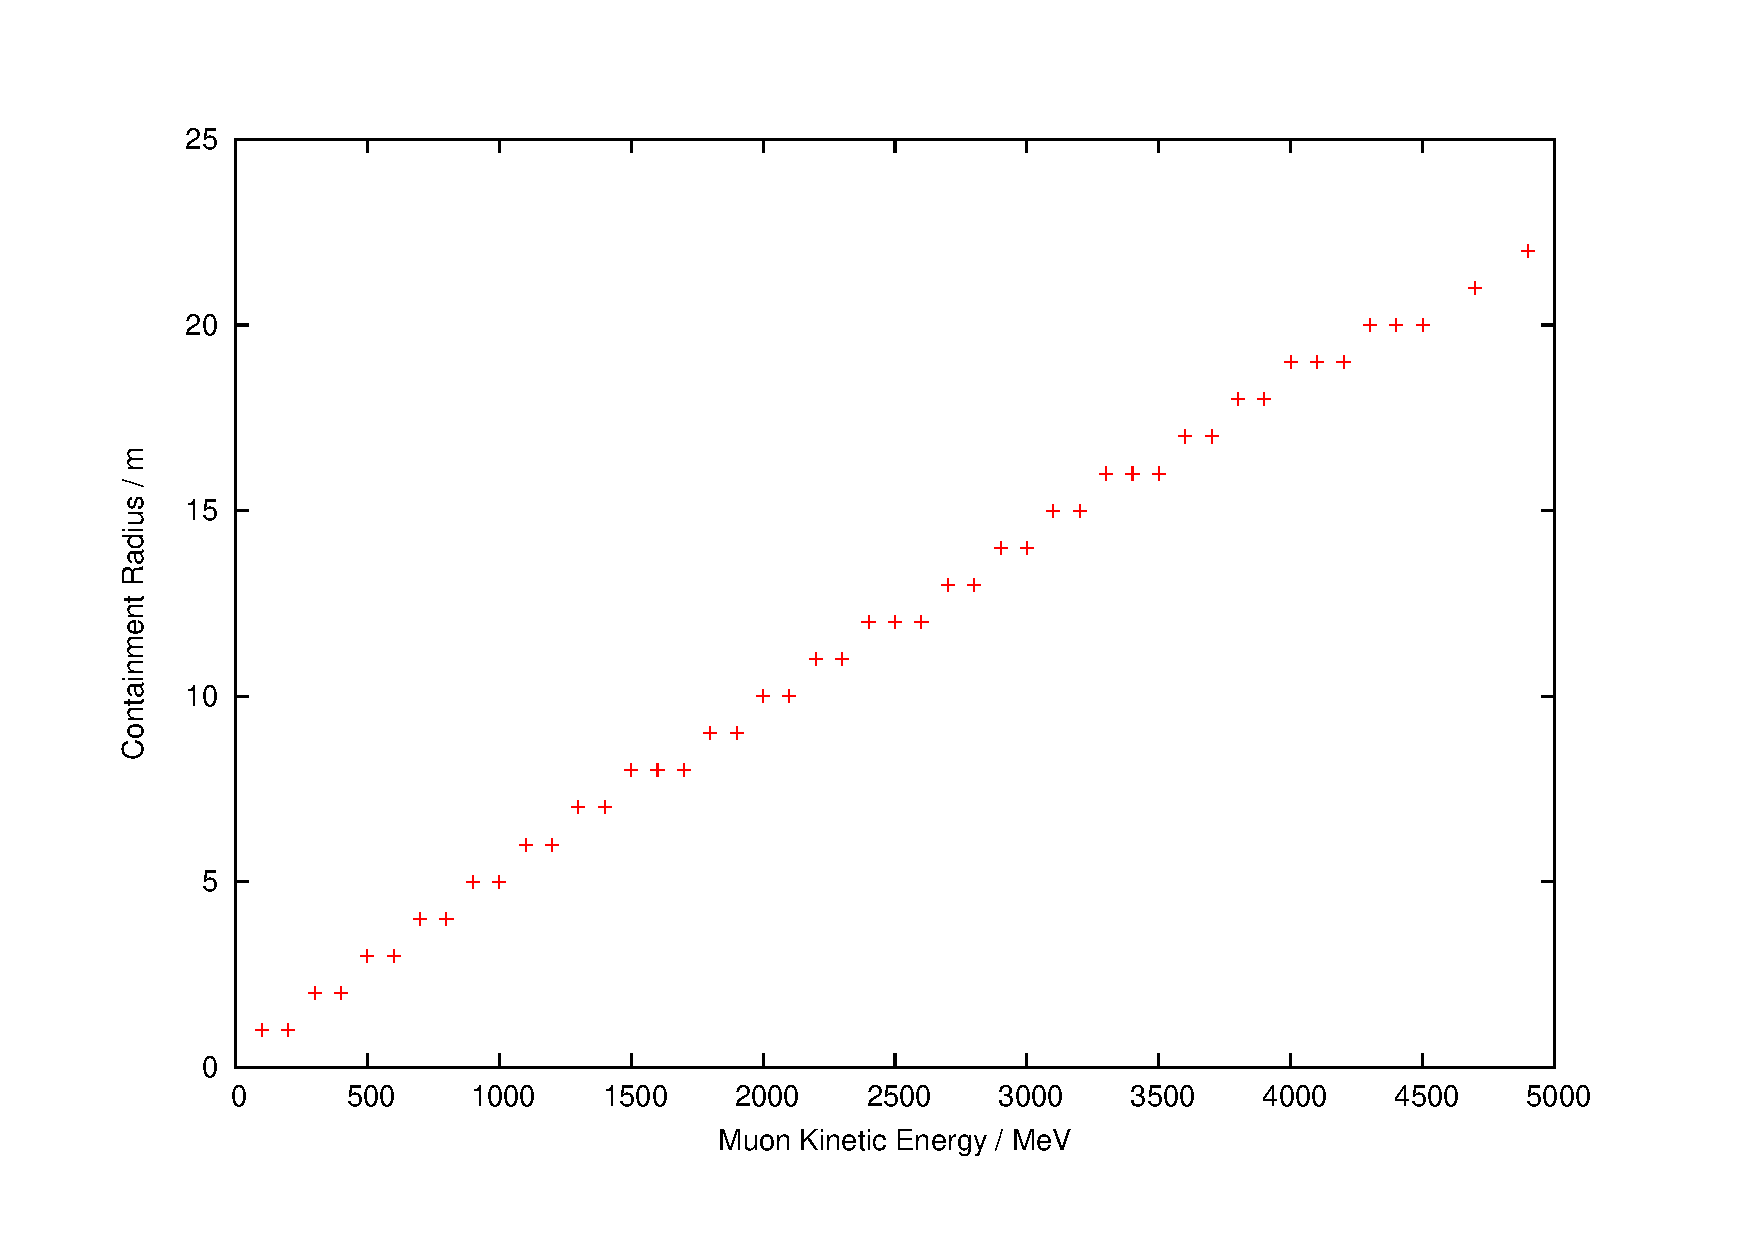
\includegraphics[angle=-90,width=0.9\textwidth]{chapters/detectorphysics_images/containment_radius}
\caption[Detector radius required for full containment as a function of energy]{\label{fig:lamu-containment-radius}Minimum detector radius required in order to fully contain muon tracks, as a function of the muon kinetic energy. This information is used to ensure that subsequent studies have fully contained primary particles.}
\end{figure}

The second test relates to the ionisation charge quenching factor built into the Lamu simulation. For this test, particles of several species were tracked through the detector with a fixed initial kinetic energy, and the total energy deposited was recorded by summing the energy deposited in each voxel. The results of this study are shown in fig. \ref{fig:detector_energy_ratios}, giving the ratio of energy deposited in the simulated \ac{LAr} volume to the initial kinetic energy of the particle. This is plotted separately for muons, protons, electrons, and charged pions.

For each plot, the calculation of energy deposited took into account only hits produced by a particle of the species under consideration. For muons, the ratio is fairly consistent with the quenching formula since a muon will behave much the same irrespective of energy (within the range considered). For protons and charged pions, the higher energy particles are more likely to undergo hadronic interactions resulting in particles of different species. In this way, the energy deposited by protons drops as the proton energy increases, since most of the energy is carried away by products of hadronic interactions. The same applies for pions.

In the case of electrons, as the energy increases, the chance of an electromagnetic shower occurring also increases in analogy to the hadronic showers of protons and charged pions. However, the ratio curve plotted in fig. \ref{fig:detector_energy_ratios_electron} does not show a significant drop since the (charged) products of an electromagnetic shower are themselves electrons, and all energy deposited by electrons was counted towards the deposition from the primary particle.

\begin{figure}
\centering
\subfigure[Muon]{
    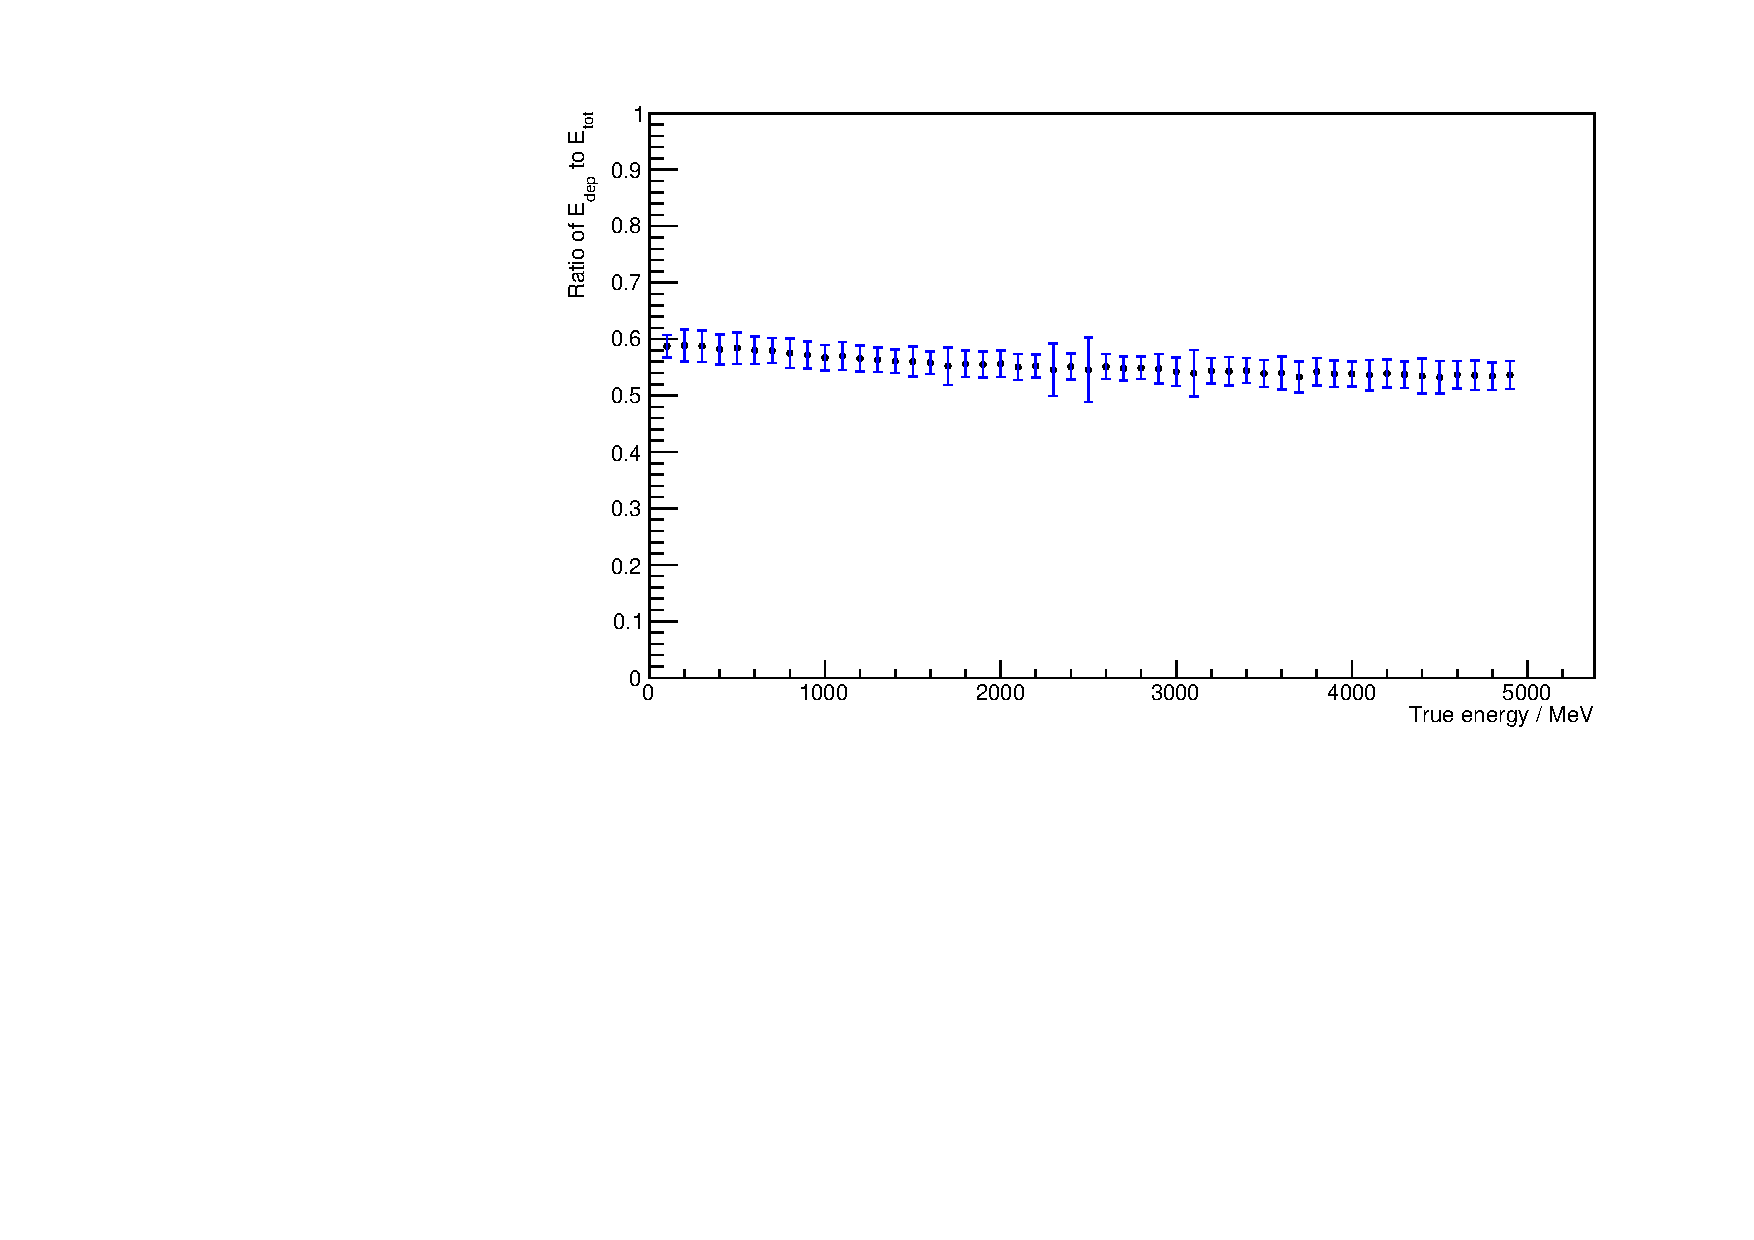
\includegraphics[angle=-90,width=0.45\textwidth]{chapters/detectorphysics_images/muon-energy-ratio}
    \label{fig:detector_energy_ratios_muon}
    }
\subfigure[Proton]{
    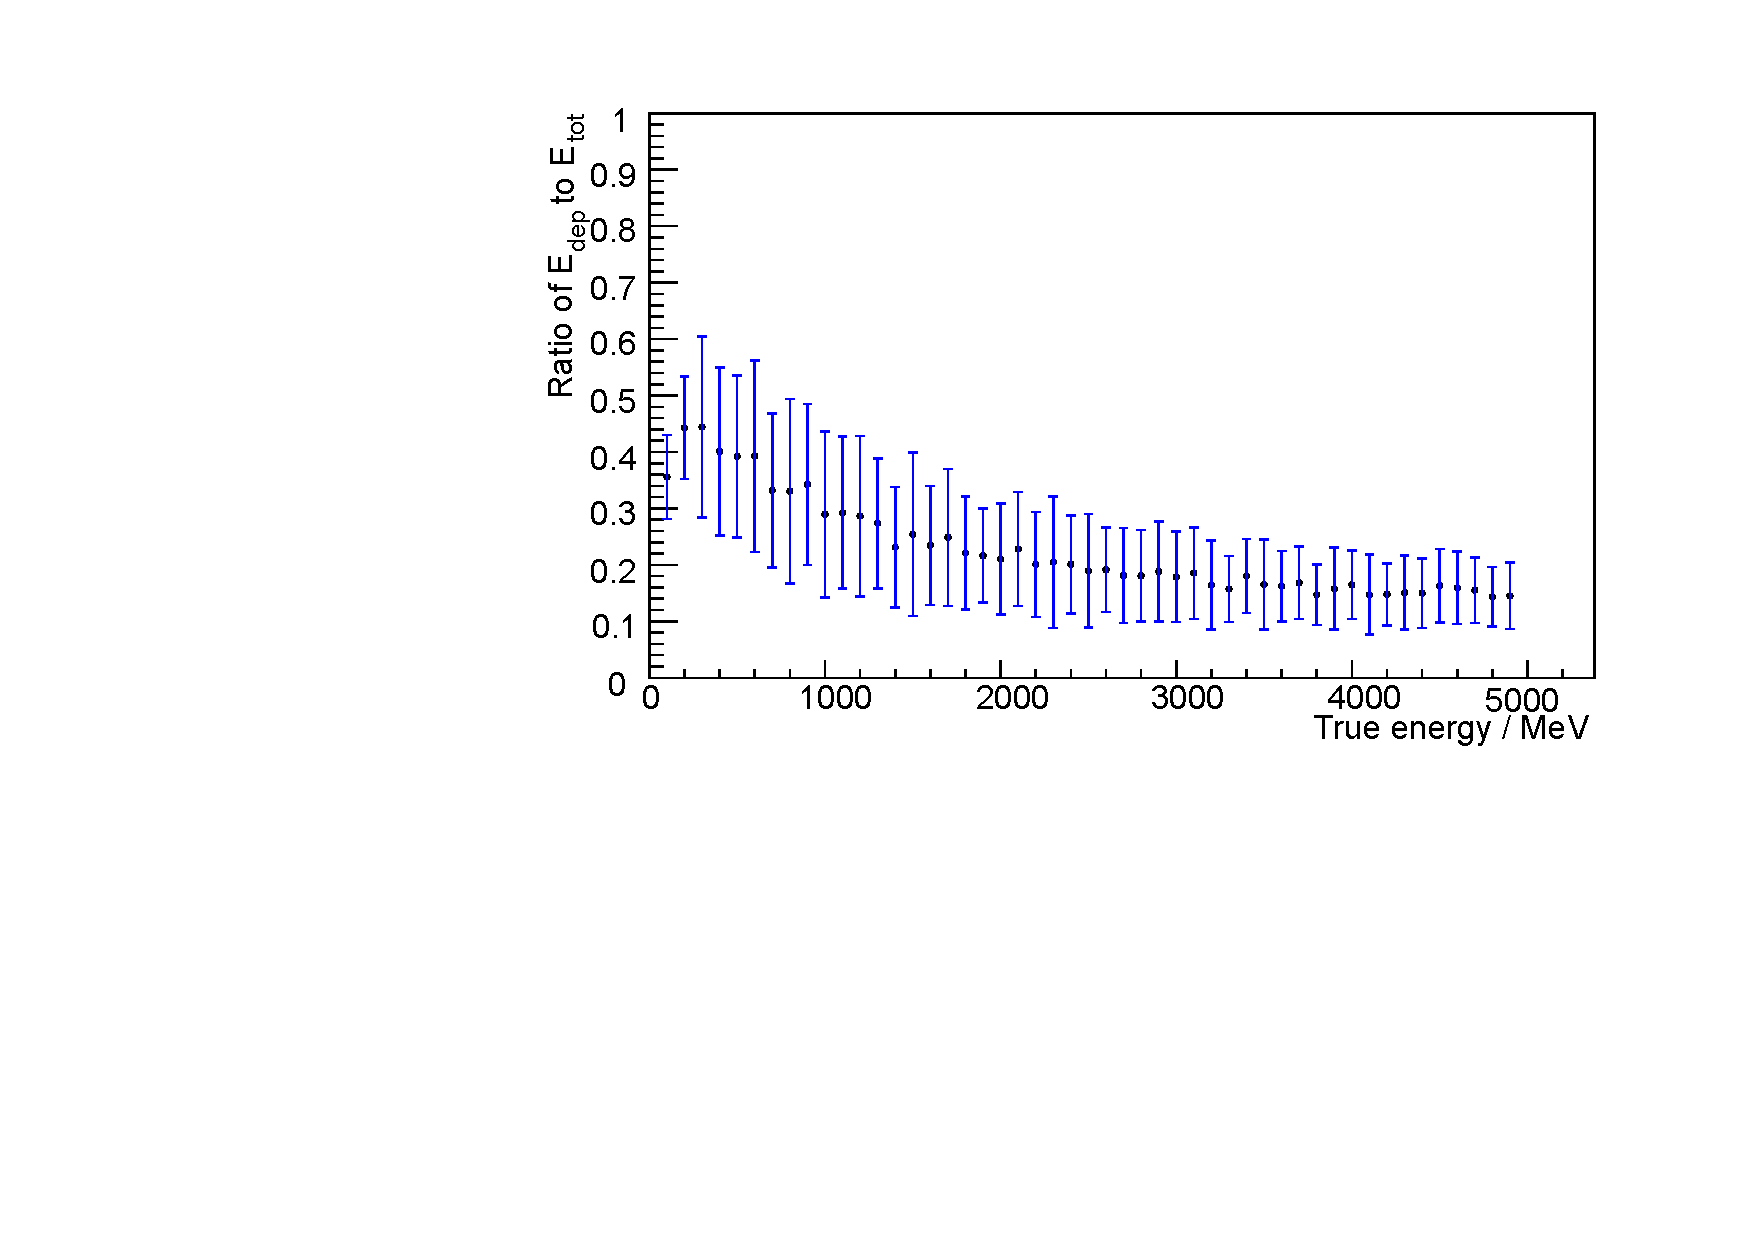
\includegraphics[angle=-90,width=0.45\textwidth]{chapters/detectorphysics_images/proton-energy-ratio}
    \label{fig:detector_energy_ratios_proton}
    }
\subfigure[Electron]{
    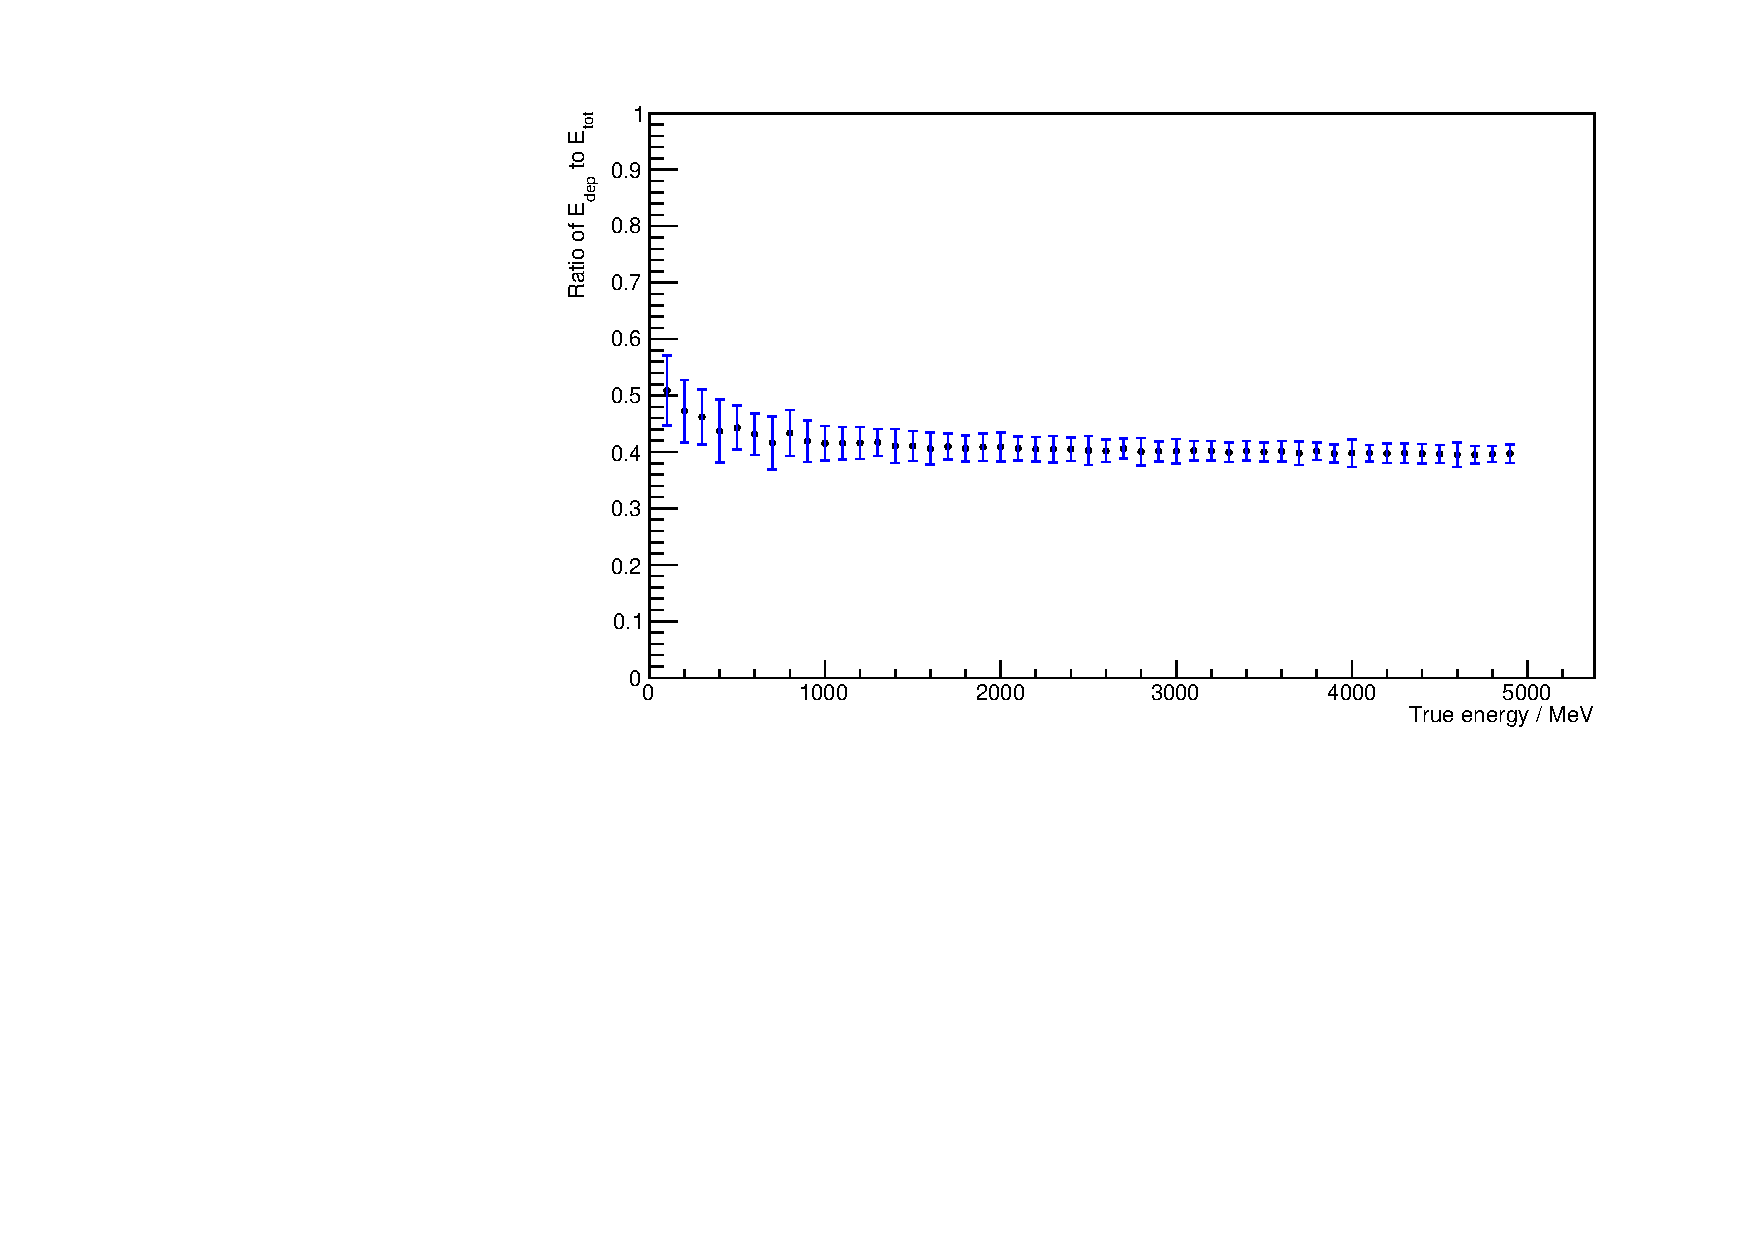
\includegraphics[angle=-90,width=0.45\textwidth]{chapters/detectorphysics_images/electron-energy-ratio}
    \label{fig:detector_energy_ratios_electron}
    }
\subfigure[Charged Pion]{
    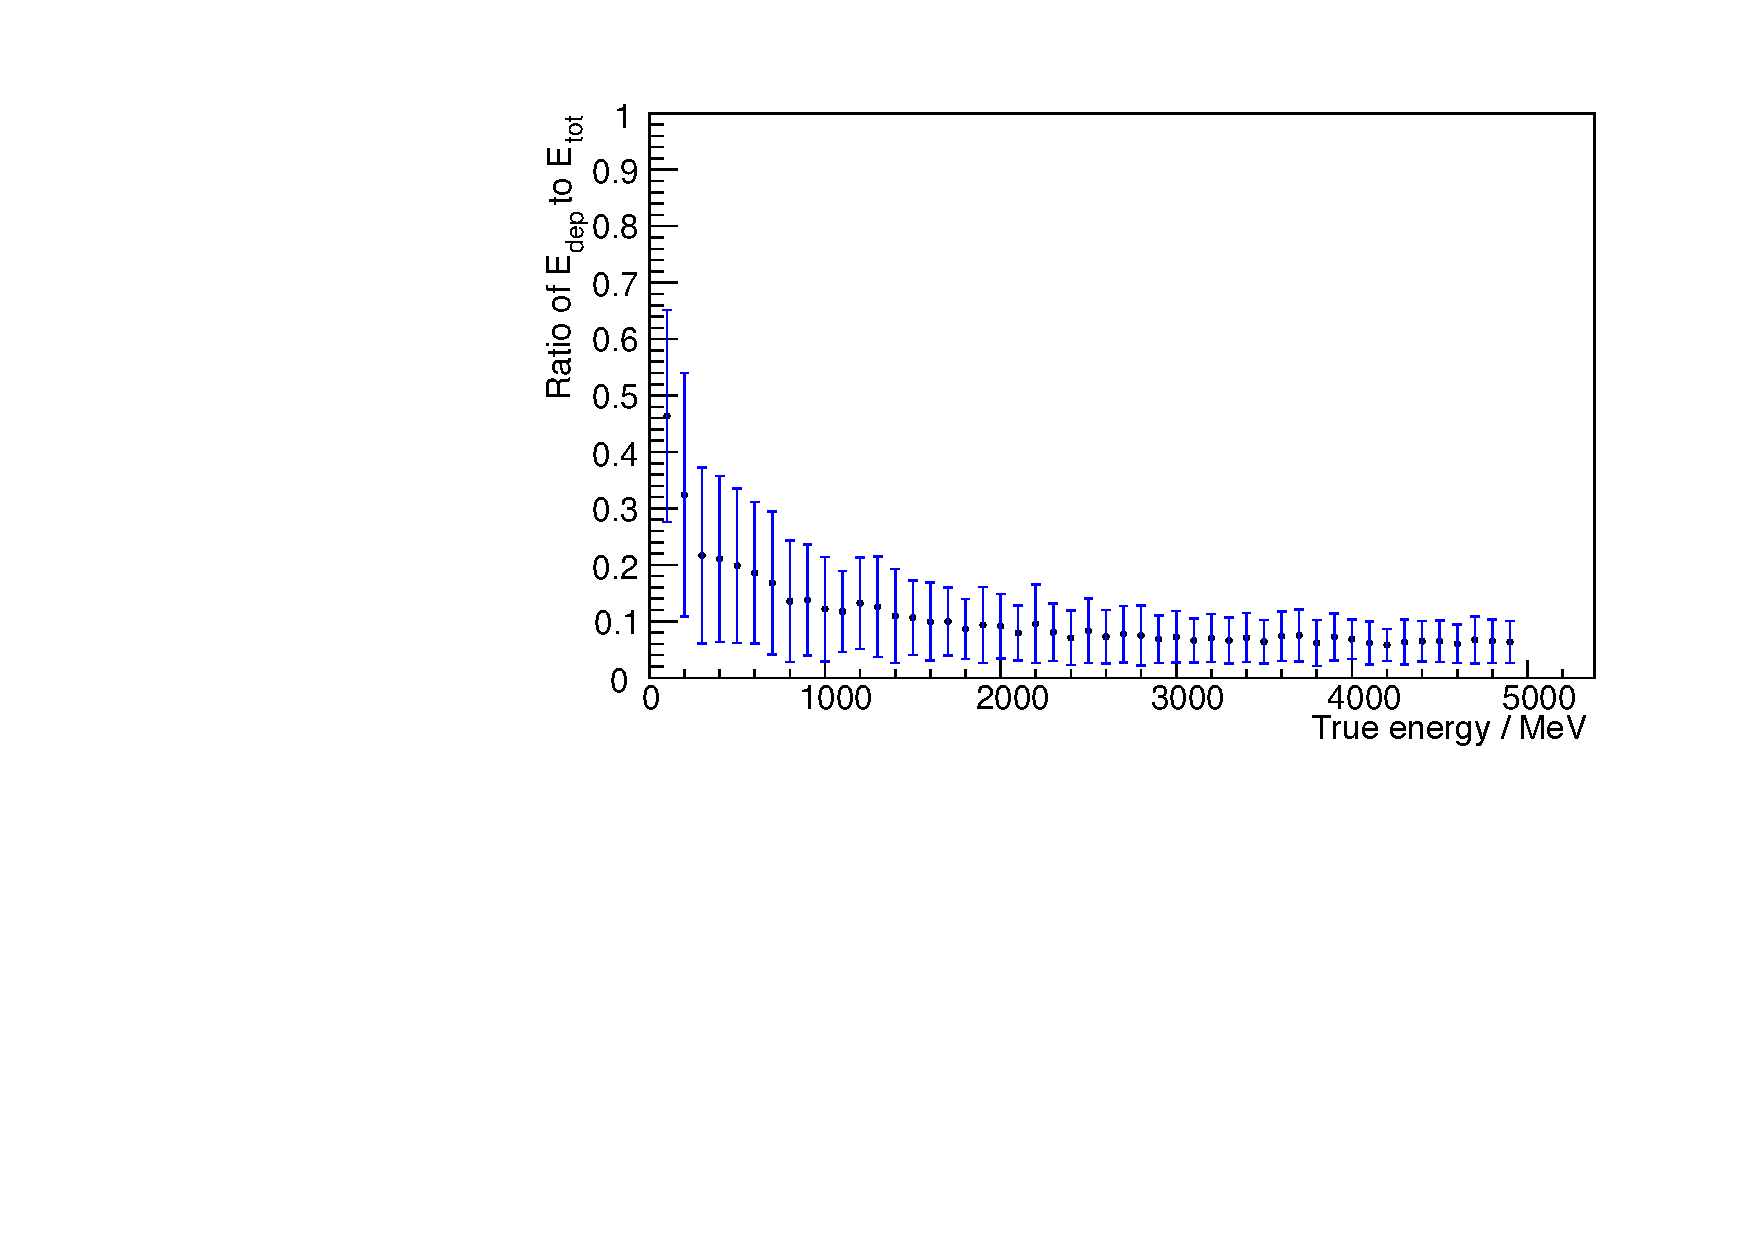
\includegraphics[angle=-90,width=0.45\textwidth]{chapters/detectorphysics_images/pi+-energy-ratio}
    \label{fig:detector_energy_ratios_charged_pion}
    }
\caption[Ratio of energy deposited to kinetic energy, by particle species]{\label{fig:detector_energy_ratios}Ratio of energy deposited in the Lamu simulation to the initial kinetic energy of the particle, by particle species. See text for discussion.}
\end{figure}

\section{The TrackGen Toy Track Simulation}
In addition to the full physics simulation provided by Lamu (see section \ref{sec:lamu}), it is useful to be able to test algorithms for event reconstruction using simplified ``toy'' tracks. The TrackGen simulation is a Python program which produces events containing one or more straight line segments, tracked through cubic voxels with ``energy'' deposition $L\cdot dE/dx$ where $L$ is the length of the track segment through a voxel and $dE/dx$ is a constant `energy loss' per unit length for the track concerned. The calculated `energy' is deposited at the centre of each voxel. There is no attempt to model physics processes such as Bethe-Bloch energy loss or scattering. Similarly, no detector properties are taken into account. This produces very clean (but still voxellised) events which, in principle, can be used to test the baseline efficiency of a reconstruction algorithm without dealing with a combination of algorithm effects and physics effects.

The core of the TrackGen simulation deals with calculating the intersection of straight lines with a set of voxels, determining the segment length through a voxel, and keeping track of the energy deposits. Several event generator modules produce different sets of straight lines, corresponding to different event topologies of interest. The topologies of most relevance to the reconstruction of neutrino events are:

\begin{enumerate}
    \item Single straight line; corresponding to a muon track without scattering.
    \item Single line with kink; corresponding to a muon track with a single large scatter.
    \item Two lines originating at a vertex, with fixed opening angle; corresponding to an interaction vertex and e.g. $\ccqe$ final state.
    \item Multiple lines originating at a vertex; corresponding to a higher-energy $\nu$ interaction producing multiple final state particles.
\end{enumerate}

The TrackGen simulation has event generator modules for each of these topologies, producing events consisting of one or more straight line segments, each tracked through a voxellised space. Output is to an SQLite3\citep{SQLite} database file with a simple table structure.

\section{Neutrino Event Generation with Genie}\label{sec:genie}
The Genie\citep{Genie} neutrino event generator is used to generate sets of final state particles (including momenta) from the interactions of neutrinos of a given flavour on Argon nuclei at a variety of energies. These final state particles are fed into the Lamu simulation as input trajectories and tracked through a \ac{LAr} volume.

Genie allows for the selection of interaction type, e.g. \ac{CCQE} scattering, but it is recommended that users limit themselves to selecting only charged current or neutral current interactions, since there is not a one-to-one mapping between physical interaction and final state topology, and physicists are mostly concerned with final state topologies. For instance, when one talks about a \ac{CCQE} event, one typically thinks of a $\ccqe$ final state. The reality is that a $\ccqe$ final state can occur in a number of ways, with \ac{CCQE} interactions a major contributor. Furthermore, a \ac{CCQE} interaction can produce other final states, particularly if the resulting nucleon undergoes further interactions in the nucleus before emerging (see figure \ref{fig:feynman-cc} for illustration). For this reason, the events generated for this thesis using Genie were made by specifying only charged or neutral current interactions, without imposing limitations on the subtype of the interaction. The results were subsequently filtered to ``cherrypick'' the topologies of interest, and a note made of the fraction of the total events generated which passed the filter. In the remainder of this thesis, the term CCQE is used, for convenience, to mean ``\emph{charged current interactions producing a $\ccqe$ final state}''.

\begin{figure}
\centering
\subfigure{
    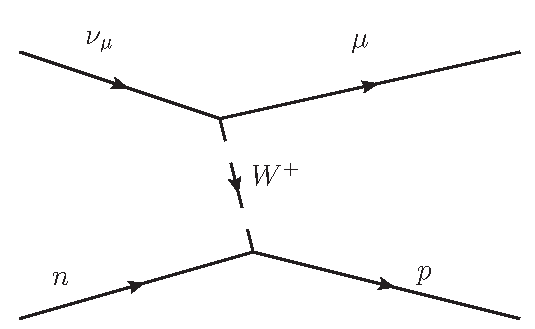
\includegraphics[width=0.45\textwidth]{chapters/detectorphysics_images/ccqe}
    \label{fig:feynman-ccqe}
}
\subfigure{
    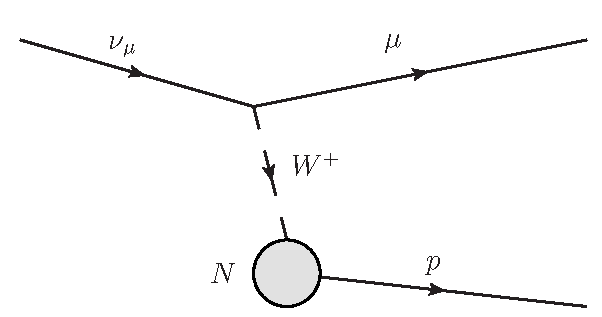
\includegraphics[width=0.45\textwidth]{chapters/detectorphysics_images/cc-mu-p}
    \label{fig:feynman-cc-mu-p}
}
\caption[Charged current neutrino interactions producing a $\ccqe$ final state]{\label{fig:feynman-cc}The difference between true charged current quasi-elastic (CCQE) interactions (left), and charged current interactions producing a $\ccqe$ final state (right). The left-hand diagram is included in the possibilities for the right-hand diagram, but in a more general sense any interaction could occur in the nucleus, and we see only the products that leave. Genie allows us to select events based on these products, leaving the details of the interaction that produced them to be decided by Genie itself.}
\end{figure}
